\section{Justificativa e Aplicações}

%A aplicação de um sistema de visão computacional requer uma boa interpretação da
%imagem, onde a informação contida nela é bastante abrangente, porém de difícil
%acesso. 

Processos mais simples como segmentação, detecção de bordas, e extração de
características locais já são amplamente utilizados em aplicações baseadas em
imagem, mas no caso da navegação robótica em ambientes não estruturados é
necessário o uso de informações de percepção espacial (3D), a fim de identificar
obstáculos e outros elementos que possam prejudicar a navegação do robô.
Com a capacidade de processamento dos computadores atuais, algoritmos mais
complexos e custosos se tornam viáveis, permitindo a concepção de um sistema de
visão computacional mais eficaz. Com o uso de câmeras estéreo associadas com
técnicas para a geração dos mapas de disparidade é possível obter, a partir
deste tipo de câmeras, dados semelhantes aos sensores do tipo
\textit{rangefinder}, baseados em sonar, laser (LIDAR - \textit{Light Detection
And Ranging}) ou infravermelho, porém com uma resolução espacial superior na
ordem de \textit{megapixels}. Além disto, as câmeras são dispositivos de baixo
custo se comparadas, por exemplo, com dispositivos como os sensores a laser de
medida de distância. Até mesmo as câmeras estéreo possuem atualmente um custo
relativamente baixo em relação a estes tipos de sensores pois a princípio são
constituídas a partir de duas câmeras comuns.

Uma das principais motivações deste trabalho advém da possibilidade de uma
aplicação conforme apresentada em um estudo anterior desenvolvido em
\cite{Pessin2008}, onde foi desenvolvido um sistema multiagente de robôs móveis
com a finalidade de combate a incêndios florestais em um ambiente simulado. Os
veículos simulados foram equipados com sonares (ou sensores laser do tipo
LIDAR), bússola e GPS para permitir a navegação autônoma em ambientes externos
não estruturados (\textit{outdoor} e \textit{off-road}). O ambiente adotado foi
tipicamente uma floresta, ou mata não muito densamente ocupada, que permitia o
deslocamento daqueles veículos. Naquele trabalho foi demonstrado com sucesso o
uso de uma Rede Neural Artificial (RNA) treinada para controlar o veículo,
integrando os dados sensoriais e a geração de comandos para os atuadores do
mesmo. Estes veículos robóticos autônomos, denominados de
RoBombeiros\foot{RoBombeiros – Site com material referente ao projeto:
http://sites.google.com/site/pessin}, são capazes de se deslocar em direção ao
foco de incêndio desviando de obstáculos e aproximando do local estimado, onde
devem realizar as ações de combate ao fogo \cite{Pessin2007, Pessin2010}.
Esta abordagem servirá de base e inspiração para o projeto e aplicação do
sistema de controle de navegação que será então desenvolvido, porém será adotado
um sistema de visão computacional como principal informação sensorial e a
utilização de um veículo terrestre real.
% Outra importante aplicação deste trabalho que está sendo proposto é junto a
% aplicações agrícolas: máquinas e implementos agrícolas que possam se deslocar
% pelas plantações para semear, pulverizar defensivos agrícolas, arar a terra, e
% até mesmo realizar a colheita de modo autônomo.

O INCT-SEC e o LRM estabeleceram recentemente uma parceria com uma empresa
brasileira de máquinas agrícolas, a Jacto S/A\foot{Máquinas Agrícolas Jacto S/A
- http://www.jacto.com.br}\foot{Jacto - Pulverizador Autônomo JAV. Vídeo
disponível em: http://www.youtube.com/watch?v=JwTm1kQ2gE0}, cuja sede fica
situada na cidade de Pompéia/SP. A proposta desta cooperação é o desenvolvimento
de soluções robóticas para a automação de veículos agrícolas. Tais veículos
deverão poder atuar em diferentes plantações (por exemplo, café,
\textit{citrus}/laranja e cana-de-açúcar, que são culturas muito difundidas no
estado de São Paulo, e também em outros estados). Testes preliminares foram
realizados pelos membros do Laboratório LRM, demonstrando a viabilidade do uso
de um sistema de visão baseado em câmeras estéreo para uso em aplicações
agrícolas\foot{NAV-AG:
http://www.lrm.icmc.usp.br/?page=projetos\&projeto=navag}.
A \fig{fig:um} apresenta as plataformas robóticas que tem servido como base de
referência para a proposta e desenvolvimento deste projeto:
veículos simulados (RoBombeiros), veículo JAV da Jacto S/A (\textit{Jacto
Autonomous Vehicle}) e veículo automatizado dotado de câmera e atuadores para
navegação autônoma (CaRINA I, desenvolvido junto ao INCT-SEC e ao LRM-ICMC/USP).

\vspace{1cm}

\begin{figure}[!h]
  	\centering
	\begin{minipage}[b]{1.0\linewidth}
	    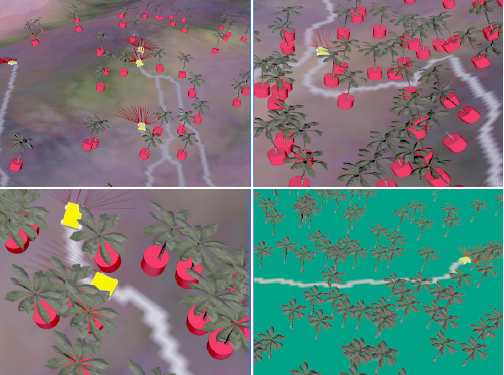
\includegraphics[width=0.33\textwidth,height=5cm]{images/robombeiros2.png}
	    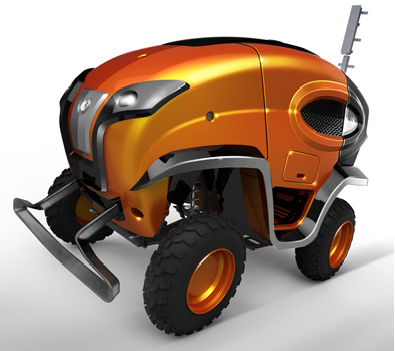
\includegraphics[width=0.33\textwidth,height=5cm]{images/jacto.png}
	    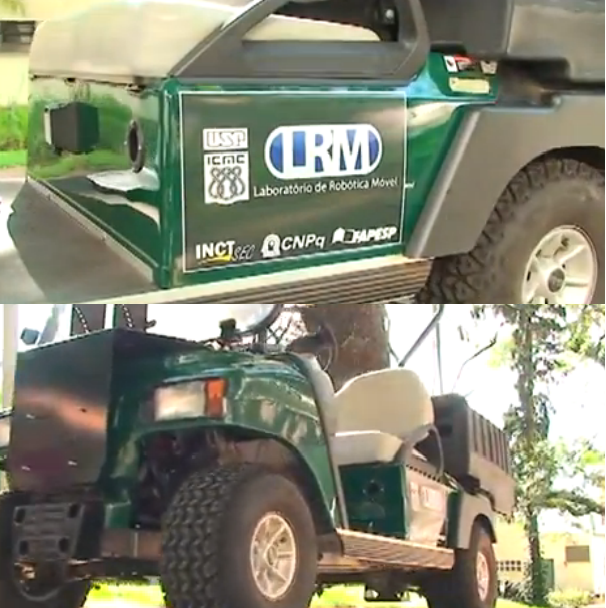
\includegraphics[width=0.33\textwidth,height=5cm]{images/carina_1_stacked.png}
	 	\caption{Simulador RoBombeiros (\textit{esquerda}), 
	 	Jacto JAV (\textit{centro}), CaRINA I (\textit{direita})}
		\fonte{(Jacto S/A, LRM–ICMC/USP)}
	 	\label{fig:um}
 	\end{minipage}
\end{figure}

%2012-10-15 Lido OK

